\documentclass[12pt]{article}
%%---------------------------------------------------------------------
% packages
% geometry
\usepackage{geometry}
% font
\usepackage{fontspec}
\defaultfontfeatures{Mapping=tex-text}  %%如果没有它,会有一些 tex 特殊字符无法正常使用,比如连字符。
\usepackage{xunicode,xltxtra}
\usepackage[BoldFont,SlantFont,CJKnumber,CJKchecksingle]{xeCJK}  % \CJKnumber{12345}: 一万二千三百四十五
\usepackage{CJKfntef}  %%实现对汉字加点、下划线等。
\usepackage{pifont}  % \ding{}
% math
\usepackage{amsmath,amsfonts,amssymb}
% color
\usepackage{color}
\usepackage{xcolor}
\definecolor{EYE}{RGB}{199,237,204}
\definecolor{FLY}{RGB}{128,0,128}
\definecolor{ZHY}{RGB}{139,0,255}
% graphics
\usepackage[americaninductors,europeanresistors]{circuitikz}
\usepackage{tikz}
\usetikzlibrary{positioning,arrows,shadows,shapes,calc,mindmap,trees,backgrounds}  % placements=positioning
\usepackage{graphicx}  % \includegraphics[]{}
\usepackage{subfigure}  %%图形或表格并排排列
% table
\usepackage{colortbl,dcolumn}  %% 彩色表格
\usepackage{multirow}
\usepackage{multicol}
\usepackage{booktabs}
\usepackage{tcolorbox}
% code
\usepackage{fancyvrb}
\usepackage{listings}
\lstset{language=C++}%这条命令可以让LaTeX排版时将C++键字突出显示
\lstset{breaklines}%这条命令可以让LaTeX自动将长的代码行换行排版
\lstset{extendedchars=false}
% title
\usepackage{titlesec}
% head/foot
\usepackage{fancyhdr}
% ref
\usepackage{hyperref}
% pagecolor
\usepackage[pagecolor={EYE}]{pagecolor}
% tightly-packed lists
\usepackage{mdwlist}

\usepackage{styles/iplouccfg}
\usepackage{styles/zhfontcfg}
\usepackage{styles/iplouclistings}

%%---------------------------------------------------------------------
% settings
% geometry
\geometry{left=2cm,right=1cm,top=2cm,bottom=2cm}  %设置 上、左、下、右 页边距
\linespread{1.5} %行间距
% font
\setCJKmainfont{Adobe Kaiti Std}
%\setmainfont[BoldFont=Adobe Garamond Pro Bold]{Apple Garamond}  % 英文字体
%\setmainfont[BoldFont=Adobe Garamond Pro Bold,SmallCapsFont=Apple Garamond,SmallCapsFeatures={Scale=0.7}]{Apple Garamond}  %%苹果字体没有SmallCaps
\setCJKmonofont{Adobe Fangsong Std}
% graphics
\graphicspath{{figures/}}
\tikzset{
    % Define standard arrow tip
    >=stealth',
    % Define style for boxes
    punkt/.style={
           rectangle,
           rounded corners,
           draw=black, very thick,
           text width=6.5em,
           minimum height=2em,
           text centered},
    % Define arrow style
    pil/.style={
           ->,
           thick,
           shorten <=2pt,
           shorten >=2pt,},
    % Define style for FlyZhyBall
    FlyZhyBall/.style={
      circle,
      minimum size=6mm,
      inner sep=0.5pt,
      ball color=red!50!blue,
      text=white,},
    % Define style for FlyZhyRectangle
    FlyZhyRectangle/.style={
      rectangle,
      rounded corners,
      minimum size=6mm,
      ball color=red!50!blue,
      text=white,},
    % Define style for zhyfly
    zhyfly/.style={
      rectangle,
      rounded corners,
      minimum size=6mm,
      ball color=red!25!blue,
      text=white,},
    % Define style for new rectangle
    nrectangle/.style={
      rectangle,
      draw=#1!50,
      fill=#1!20,
      minimum size=5mm,
      inner sep=0.1pt,}
}
\ctikzset{
  bipoles/length=.8cm
}
% code
\lstnewenvironment{VHDLcode}[1][]{%
  \lstset{
    basicstyle=\footnotesize\ttfamily\color{black},%
    columns=flexible,%
    framexleftmargin=.7mm,frame=shadowbox,%
    rulesepcolor=\color{blue},%
%    frame=single,%
    backgroundcolor=\color{yellow!20},%
    xleftmargin=1.2\fboxsep,%
    xrightmargin=.7\fboxsep,%
    numbers=left,numberstyle=\tiny\color{blue},%
    numberblanklines=false,numbersep=7pt,%
    language=VHDL%
    }\lstset{#1}}{}
\lstnewenvironment{VHDLmiddle}[1][]{%
  \lstset{
    basicstyle=\scriptsize\ttfamily\color{black},%
    columns=flexible,%
    framexleftmargin=.7mm,frame=shadowbox,%
    rulesepcolor=\color{blue},%
%    frame=single,%
    backgroundcolor=\color{yellow!20},%
    xleftmargin=1.2\fboxsep,%
    xrightmargin=.7\fboxsep,%
    numbers=left,numberstyle=\tiny\color{blue},%
    numberblanklines=false,numbersep=7pt,%
    language=VHDL%
    }\lstset{#1}}{}
\lstnewenvironment{VHDLsmall}[1][]{%
  \lstset{
    basicstyle=\tiny\ttfamily\color{black},%
    columns=flexible,%
    framexleftmargin=.7mm,frame=shadowbox,%
    rulesepcolor=\color{blue},%
%    frame=single,%
    backgroundcolor=\color{yellow!20},%
    xleftmargin=1.2\fboxsep,%
    xrightmargin=.7\fboxsep,%
    numbers=left,numberstyle=\tiny\color{blue},%
    numberblanklines=false,numbersep=7pt,%
    language=VHDL%
    }\lstset{#1}}{}
% pdf
\hypersetup{pdfpagemode=FullScreen,%
            pdfauthor={Haiyong Zheng},%
            pdftitle={Title},%
            CJKbookmarks=true,%
            bookmarksnumbered=true,%
            bookmarksopen=false,%
            plainpages=false,%
            colorlinks=true,%
            citecolor=green,%
            filecolor=magenta,%
            linkcolor=cyan,%red(default)
            urlcolor=cyan}
% section
%http://tex.stackexchange.com/questions/34288/how-to-place-a-shaded-box-around-a-section-label-and-name
\newcommand\titlebar{%
\tikz[baseline,trim left=3.1cm,trim right=3cm] {
    \fill [cyan!25] (2.5cm,-1ex) rectangle (\textwidth+3.1cm,2.5ex);
    \node [
        fill=cyan!60!white,
        anchor= base east,
        rounded rectangle,
        minimum height=3.5ex] at (3cm,0) {
        \textbf{\thesection.}
    };
}%
}
\titleformat{\section}{\Large\bf\color{blue}}{\titlebar}{0.1cm}{}
% head/foot
\setlength{\headheight}{15pt}
\pagestyle{fancy}
\fancyhf{}
%\lhead{\color{black!50!green}2014年秋季学期}
\chead{\color{black!50!green}Zooplankton Identification}
%\rhead{\color{black!50!green}通信电子电路}
\lfoot{\color{blue!50!green}王如晨\ 朱亚菲}
\cfoot{\color{blue!50!green}\href{http://vision.ouc.edu.cn/~zhenghaiyong}{CVBIOUC}}
\rfoot{\color{blue!50!green}$\cdot$\ \thepage\ $\cdot$}
\renewcommand{\headrulewidth}{0.4pt}
\renewcommand{\footrulewidth}{0.4pt}


%%---------------------------------------------------------------------
\begin{document}
%%---------------------------------------------------------------------
%%---------------------------------------------------------------------
% \titlepage
\title{\vspace{-2em}浮游动物识别\vspace{-0.7em}}
\author{王如晨\ 朱亚菲}
\date{\vspace{-0.7em}2015年7月\vspace{-0.7em}}
%%---------------------------------------------------------------------
\maketitle\thispagestyle{fancy}
%%---------------------------------------------------------------------
\maketitle
\tableofcontents 



\section{竞赛}


\subsection{PASCAL VOC Challenges 2005-2012}

PASCAL VOC挑战赛是视觉对象的分类识别和检测的一个基准测试,提供了检测算法和学习性能的标准图像注释数据集和标准的评估系统。

挑战赛主要分为三个部分:图像的分类、识别、分割,另外还有一个“动态”分类项目,一个由Image Net 举行的大规模识别竞赛和人类身体部位识别的附加赛项目。

分类就是让算法找出测试图片都是属于哪一个标签,对测试的图片进行分类,将图片对号入座。检测则是检测出测试图片中由委员会特别圈定的内容,看看算法能否正确的符合圈定的内容。分割是对图片进行像素级分割,也就是识别出的特定物体用一种颜色表示,其他的则作为背景。动作分类则是在静态图片中预测人类的动作,比如有一张人类跑步的图片,算法根据身体各部位的位置特征判别这个动作是“running”。人类轮廓识别就是识别标示出来的人体部位,这对于一张图片有多个人或者两个人身体部分纠缠在一起的图片识别有重要意义。

\subsection{IMAGENET Large Scale Visual Recognition Challenges 2010-2015}

ILSVRC每年的竞赛内容包括:

\begin{itemize}
\item ILSVRC2014: {\color{blue}Detection} and {\color{blue}Classification and localization}
\item ILSVRC2013: {\color{blue}Detection} and {\color{blue}Classification and localization}
\item ILSVRC2012: {\color{blue}Classification}, {\color{blue}Classification and localization} and {\color{blue}Fine-grained classification}
\item ILSVRC2011: {\color{blue}Classification} and {\color{blue}Classification and localization}
\item ILSVRC2010: {\color{blue}Classification}
\end{itemize}

\subsection{Labeled Faces in the Wild}

\section{特征(Ours)}

\subsection{经典特征}

\subsubsection{SIFT特征}

SIFT(Scale invariant feature transform,尺度不变特征变换)是一种检测局部特征的算法,该算法通过求得一幅图像中的特征点及有关尺度和方向的描述子得到特征并进行图像特征点匹配,它由 David Lowe 在 1999 年~\cite{lowe1999object}所发表, 2004 年~\cite{lowe2004distinctive}完善总结。%SIFT算法提取的特征点具有尺度不变性,也就是说,同一物体在图像上不论尺度大小,都能根据SIFT算法提取到相同的特征点。

{\color{blue}主要思想}:SIFT算法是一种提取局部特征的算法,在尺度空间寻找极值点,提取位置、尺度、旋转不变量。

{\color{blue}算法步骤}:

\begin{enumerate}
\item 构建尺度空间,检测极值点,获得尺度不变性。
    
    通过高斯微分函数来识别潜在的对于尺度和旋转不变的兴趣点。用不同尺度(标准差)的高斯函数对图像进行平滑,然后比较平滑后图像的差别,差别大的像素就是特征明显的点。
    
    原始图像经过不同尺度的高斯模糊所得的一组图像空间定义为:
    \begin{displaymath}
        L(x,y,\sigma)=G(x,y,\sigma)*I(x,y)
    \end{displaymath}
    
    其中$I(x,y)$是原始图像,$\sigma$大小决定图像的平滑程度,$G(x,y,\sigma)$是尺度可变高斯函数:
    \begin{displaymath}
        G(x,y,\sigma)=\frac{1}{2\pi \sigma^{2}}e^{\frac{-(x^{2}+y^{2})}{2\sigma^{2}}}
    \end{displaymath}
    
    为了有效地在尺度空间检测到稳定的关键点,提出了高斯差分尺度空间。利用 不同尺度的高斯差分核与图像卷积生成。
    \begin{displaymath}
        D(x,y,\sigma)=[G(x,y,k\sigma)-G(x,y,\sigma)]*I(x,y)=L(x,y,k\sigma)-L(x,y,\sigma)
    \end{displaymath}
    
\item 精确定位出特征关键点的位置。

\item 为关键点指定方向参数。

利用关键点邻域像素的梯度方向分布特性,我们可以为每个关键点指定方向参数方向,从而使描述子对图像旋转具有不变性,我们通过求每个极值点的梯度来为极值点赋予方向。
\begin{displaymath}
    m(x,y)=\sqrt{[L(x+1,y)-L(x-1,y)]^{2}+[L(x,y+1)-L(x,y-1)]^{2}}
\end{displaymath}
\begin{displaymath}
    \theta(x,y)=\alpha\tan2\frac{L(x,y+1)-L(x,y-1)}{L(x+1,y)-L(x-1,y)}
\end{displaymath}

方向直方图的生成:确定关键点的方向采用梯度直方图统计法,统计以关键点为原点,一定区域内的图像像素点对关键点方向生成所做的贡献。梯度直方图的范围是0~360度,其中每45度一个柱,总共8个柱。以特征点为中心取$16\times16$的邻域作为采样窗口,将采样点与特征点的相对方向通过高斯加权后归入包含8个bin的方向直方图,最后获得$4\times4\times8$的128维特征描述子。$16\times16$的图中其中1/4的特征点梯度方向及scale,图\ref{fig:eight}为其加权到8个主方向后的效果。
        \begin{figure}
            \centering
            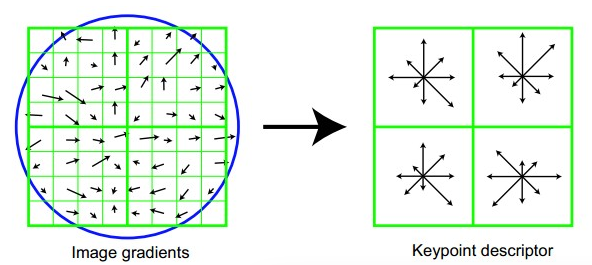
\includegraphics[width=0.5\linewidth]{sift1}
            \caption{}
            \label{fig:eight}
        \end{figure}
        
描述子采用$4\times4\times8=128$维向量表征,综合效果最优。
        \begin{figure}
            \centering
            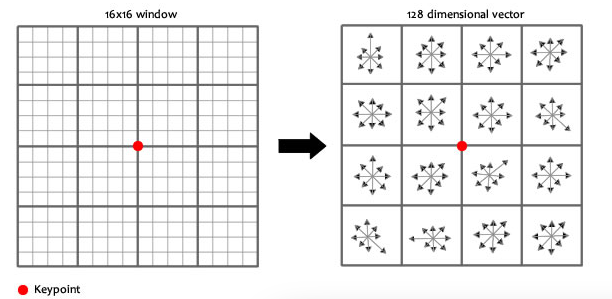
\includegraphics[width=0.5\linewidth]{sift2}
%            \caption{矩形区间和环形区间}
%            \label{fig:shape}
        \end{figure}

\item 关键点描述子产生。
\begin{enumerate}
    \item 确定计算描述子所需的图像区域,图像区域的半径通过下式计算:
        \begin{displaymath}
        radius=\frac{3\theta\_oct \times \sqrt{2} \times (d+1)}{2}
        \end{displaymath}
    \item 将坐标移至关键点主方向,如图\ref{fig:yi}。
            \begin{figure}
            \centering
            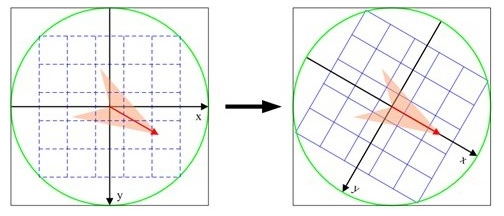
\includegraphics[width=0.5\linewidth]{yi}
            \caption{将坐标移至关键点主方向}
            \label{fig:yi}
        \end{figure}
        
        旋转后邻域内采样点的新坐标为:
        \begin{displaymath}
            \left( \begin{array}{c}
            x^{'} \\
            y^{'} \\
            \end{array} \right)
            =\left( \begin{array}{cc}
            \cos\sigma & -\sin\sigma \\
            \sin\sigma & \cos\sigma \\
            \end{array} \right)
             \left( \begin{array}{c}
            x \\
            y \\
            \end{array} \right)
        \end{displaymath}
        \item 在图像半径区域内对每个像素点求其梯度幅值和方向,然后对每个梯度幅值乘以高斯权重参数,生成方向直方图。
        \item 在窗口宽度为$2 \times 2$的区域内计算8个方向的梯度方向直方图,绘制每个梯度方向的累加值,即可形成一个种子点。然后再在下一个$2 \times 2$的区域内进行直方图统计,形成下一个种子点,共生成16个种子点。
        \item 描述子向量元素门限化及门限化后的描述子向量规范化。
        \item 根据特征点的尺度对特征描述向量进行排序,SIFT特征向量生成.
\end{enumerate}
\end{enumerate}

{\color{blue}应用}:

特征点检测匹配

{\color{blue}代码}:

采用vl\_feat中的sift特征函数:
    \begin{lstlisting}[language=C++]
    [f,d] = vl_sift(img);
    \end{lstlisting}

\subsubsection{HOG特征}

HOG~\cite{dalal2005histograms}(Histogram of Oriented Gradients,方向梯度直方图)是一种在计算机视觉和图像处理中用来进行物体检测的特征描述子,它通过统计图像局部区域的梯度方向直方图来构成特征。HOG特征结合\textbf{SVM分类器}已经被广泛应用于图像识别中,尤其在\textbf{行人检测}中获得了极大的成功。

{\color{blue}主要思想}:局部目标的表象和形状能够被梯度或边缘的方向密度分布很好地描述。
%首先计算图片中不同方向上的梯度值,然后将图像分成小的连通区域,我们把它叫细胞单元(cell),采集细胞单元中各像素点的梯度或边缘的方向直方图,这个直方图就可以代表这块区域的特征。

{\color{blue}具体实现方法}:将图像分成小的连通区域,我们把它叫细胞单元(cell)。然后采集细胞单元中各像素点的梯度的或边缘的方向直方图,最后把这些直方图组合起来就可以构成特征描述器。具体实现流程如图\ref{fig:shixian}。
        \begin{figure}
            \centering
            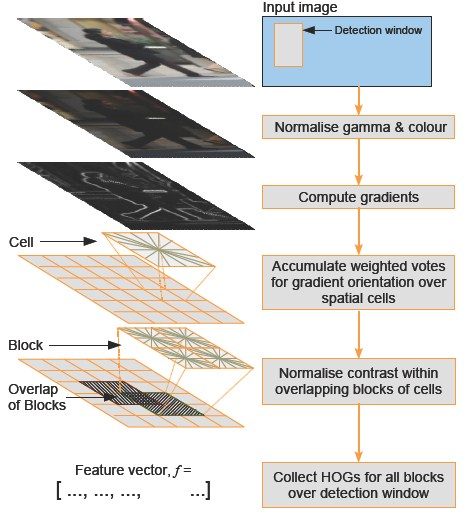
\includegraphics[width=0.4\linewidth]{flowchart}
            \caption{HOG特征}
            \label{fig:shixian}
        \end{figure}

{\color{blue}算法步骤}:

\begin{enumerate}
\item 图像归一化。采用 Gamma 校正法对输入图像进行颜色空间的标准化 ;目的是调节图像的对比度,降低图像局部的阴影和光照变化所造成的影响,同时可以抑制噪音的干扰。

Gamma压缩公式:
\begin{displaymath}
    I(x,y)=I(x,y)^{gamma}
\end{displaymath}

比如可以取Gamma=$\frac{1}{2}$。

\item 利用一阶微分计算每一个像素的梯度(包括大小和方向);目的是为了捕获轮廓信息,同时进一步弱化光照的干扰。
    
    采用模板$[-1~0~1]$(实验表明采用模板$[-1~0~1]$求得的梯度效果最好)计算水平和垂直方向的梯度:
        \begin{displaymath}
        G_{h}(x,y)=f(x+1,y)-f(x-1,y)~~~~\forall x,y
        \end{displaymath}
        \begin{displaymath}
        G_{v}(x,y)=f(x,y+1)-f(x,y-1)~~~~\forall x,y
        \end{displaymath}
        
        计算梯度值和梯度方向:
        \begin{displaymath}
        M(x,y)=\sqrt{G_{h}(x,y)^{2}+G_{v}(x,y)^2}
        \end{displaymath}
        \begin{displaymath}
        \theta(x,y)=\arctan\frac{G_{h}(x,y)}{G_{v}(x,y)}
        \end{displaymath}
        
\item 将图像划分成小cells(例如$6 \times 6$像素/cell)。

\item 统计每个cell的梯度直方图,可形成每个cell的描述子;
        
        构建每个单元的梯度方向直方图,将cell的梯度方向360度根据需要分成m个bin,例如图\ref{fig:bin}分成了16个bin。然后根据每个像素点的梯度方向,采用加权投票的方式得到直方图,即每一票都是带权值的,这个权值是根据该像素点的梯度幅度计算出来的。
        \begin{figure}
            \centering
            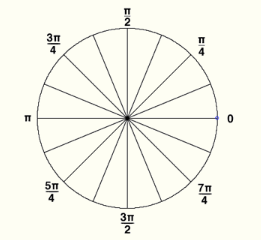
\includegraphics[width=0.3\linewidth]{bin}
            \caption{梯度方向bin}
            \label{fig:bin}
        \end{figure}
       % 一张图像由若干个块(Block)组成,一个块(Block)都由若干单元(Cell)组成,一个单元都有若干个像素点组成。块与单元的关系如图\ref{fig:block}。
       
\item 将每几个cell组成一个块(block)(例如$3 \times 3 $个cell/block),一个block内所有cell的梯度直方图串联起来便得到该block的HOG特征描述子。
    
    把各个细胞单元组合成大的、空间上连通的区间(blocks)。这样以来,HOG描述器就变成了由各区间所有细胞单元的直方图成分所组成的一个向量。这些区间是互有重叠的,这就意味着:每一个细胞单元的输出都多次作用于最终的描述器。区间有两个主要的几何形状——矩形区间(R-HOG)和环形区间(C-HOG)如图\ref{fig:shape}。
        \begin{figure}
            \centering
            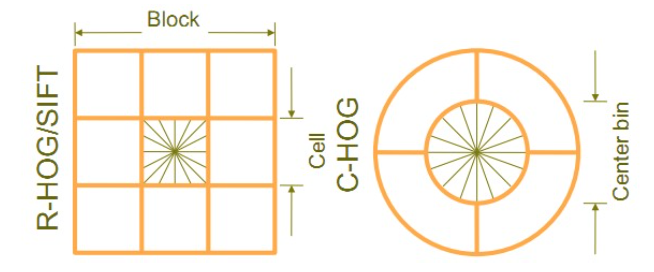
\includegraphics[width=0.5\linewidth]{shape}
            \caption{矩形区间和环形区间}
            \label{fig:shape}
        \end{figure}
        
\item 将图像内的所有block的HOG特征直方图串联起来就可以得到该图像的HOG特征描述子了。这个就是最终的可供分类使用的特征向量了。
    \begin{comment}
    对block块内特征向量的归一化主要是为了使特征向量空间对光照,阴影和边缘变化具有鲁棒性。作者采用了四中不同的方法对区间进行归一化,并对结果进行了比较。引入$v$表示一个还没有被归一化的向量,它包含了给定区间(block)的所有直方图信息。$||v_{k}||$表示v的k阶范数,这里的$k$为1、2。用$\varepsilon$表示一个很小的常数。这时,归一化因子可以表示如下:
    \begin{displaymath}
    L_{2}-norm, v \gets \frac{v}{\sqrt{||v||_{2}^{2}+\varepsilon^{2}}}
    \end{displaymath}
    \begin{displaymath}
    L_{2}-Hys% $(方法同上,只是限制v的最大值到0.2,然后再次重新标准化)$
    \end{displaymath}
    \begin{displaymath}
    L_{1}-norm, v \gets \frac{v}{||v||_{1}+\varepsilon}
    \end{displaymath}
    \begin{displaymath}
    L_{1}-sqrt, v \gets \frac{v}{\sqrt{||v||_{1}+\varepsilon}}
    \end{displaymath}
    \end{comment}

    最终可以得到一个$m \times n \times \alpha$个数据组成的高维向量,其中$m$表示每个cell中方向bin的数目,$n,\alpha$分别表示block的个数以及一个block中cell的数目。
\end{enumerate}

{\color{blue}在行人检测中的应用}:

用一个窗口(OpenCV采用$64 \times 128$)在图像中滑动,计算窗口对应的HOG特征。窗口中块的大小为$16 \times 16$,块的步长为$8 \times 8$,单元的大小为$8 \times 8$。把每一个胞元投影到9个bin,那么每一个单元对应的向量就是9维,每个bin对应该9维向量的一个数。该窗口特征向量的维数为:$9 \times \frac{16}{8} \times \frac{16}{8} \times (\frac{64-16}{8}+1) \times (\frac{128-16}{8}+1)=3780$。

{\color{blue}代码}:

采用vl\_feat中的HOG特征函数:
    \begin{lstlisting}[language=C++]
    HOG = vl_hog(img, cellsize);//img表示输入的图像,cellsize为单元的大小
    image = vl_hog('render', hog);//将HOG特征转换为图像
    \end{lstlisting}
    
{\color{blue}应用(Deformable Part Model)}:DPM是一个非常成功的目标检测算法,连续获得VOC(Visual Object Class)07、08、09年的检测冠军。目前已成为众多分类器、分割、人体姿态和行为分类的重要部分。2010年Pedro Felzenszwalb被VOC授予"终身成就奖"。DPM可以看做是HOG(Histogrrams of Oriented Gradients)的扩展,大体思路与HOG一致。先计算梯度方向直方图,然后用SVM(Surpport Vector Machine )训练得到物体的梯度模型(Model)。有了这样的模板就可以直接用来分类了,简单理解就是模型和目标匹配。DPM只是在模型上做了很多改进工作。


  
\subsubsection{SURF}

SURF与SIFT算法相似,SIFT算法比较稳定,检测特征点更多,但是复杂度较高,而SURF要运算简单,效率高,运算时间短一点。

{\color{blue}算法步骤}:

\begin{enumerate}
\item 构建Hessian矩阵。采用的是Hessian矩阵行列式近似值图像。

\item 构造多尺度空间。

为了实现尺度不变性的特征点检测与匹配,SURF算法与SIFT算法的第一步都是构造图像多尺度空间。SURF算法则用高斯滤波与Hessian矩阵结合近似实现多尺度空间,计算复杂度相比SIFT降低多了。

\item 根据非极大值抑制初步确定特征点。

\item 主方向确定

\item 构造特征点算术描述子,SURF算法是选取一个20S(单位)的区域,分成$4 \times 4$分,每一份中有$5 \times 5$S,统计一份中的$\sum d_{x}$,$\sum d_{y}$,$\sum |d_{x}|$,$\sum |d_{y}|$,这样就得到$4 \times 4 \times 4 = 64$的向量描述子。SIFT是128个描述子,比SURF复杂一点。
\end{enumerate}

\subsubsection{LBP}

LBP(Local Binary Pattern,局部二值模式)\footnote{\url{http://blog.csdn.net/zouxy09/article/details/7929531}}是一种用来描述图像局部纹理特征的算子;它具有旋转不变性和灰度不变性等显著的优点。它是首先由T. Ojala, M.Pietikäinen, 和 D. Harwood 在1994年提出~\cite{ojala1994performance},用于纹理特征提取。而且,提取的特征是图像的局部的纹理特征。
 
 原始的LBP算子定义为在$3\times3$的窗口内,以窗口中心像素为阈值,将相邻的8个像素的灰度值与其进行比较,若周围像素值大于中心像素值,则该像素点的位置被标记为1,否则为0。这样,$3\times3$邻域内的8个点经比较可产生8位二进制数(通常转换为十进制数即LBP码,共256种),即得到该窗口中心像素点的LBP值,并用这个值来反映该区域的纹理信息。如下图\ref{fig:lbp}:
    \begin{figure}[!ht]
    \centering
    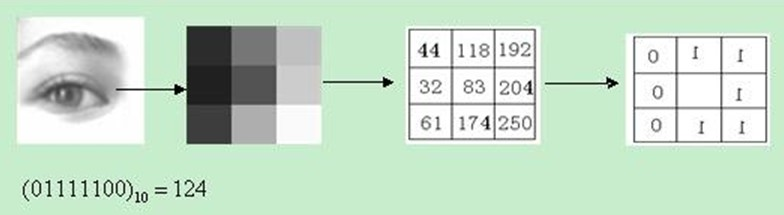
\includegraphics[width=4in]{LBP}
    \caption{LBP特征}
    \label{fig:lbp}
    \end{figure}
   
对LBP特征向量进行提取的步骤:
\begin{enumerate}
    \item 首先将检测窗口划分为$16\times16$的小区域(cell);
    \item 对于每个cell中的一个像素,将相邻的8个像素的灰度值与其进行比较,若周围像素值大于中心像素值,则该像素点的位置被标记为1,否则为0。这样,$3\times3$邻域内的8个点经比较可产生8位二进制数,即得到该窗口中心像素点的LBP值;
    \item 然后计算每个cell的直方图,即每个数字(假定是十进制数LBP值)出现的频率;然后对该直方图进行归一化处理。
    \item 最后将得到的每个cell的统计直方图进行连接成为一个特征向量,也就是整幅图的LBP纹理特征向量;
    \item 然后便可利用SVM或者其他机器学习算法进行分类了。
\end{enumerate}

\subsubsection{FV(Fisher vector)}
   
Fisher vector本质上是用似然函数的梯度vector来表达一幅图像。

{\color{blue}主要思路}:用生成式模型(GMM)对样本输入进行建模,进而得到样本的一种表示(fisher vector),再将这种表示(fisher vector)输入判别式分类器(SVM)得到图像分类结果。fisher vector是fisher kernel中对样本特征的一种表示,它把一幅图片表示成一个向量。在高斯分布的基础上再找到变化的方向,可以更加准确的表示这一张图。

{\color{blue}应用}:图像的分类,目标识别等领域,特别是结合着BOW model。

\subsubsection{骨架特征}

理论:骨架又称为中轴,它的定义来自于烧草模型和最大圆盘模型。骨架不仅包含了物体的几何特征,也描述了物体的拓扑结构。经典的骨架化算法有中轴变换、细化算法、Voronoi图算法等。在骨架的基础上可以通过奇点图、骨架树等对物体的结构特征进行描述。

骨架树:将骨架映射到一个树状结构(如图\ref{fig:tree})。仅有一个邻接点的骨架点成为端点,有两个以上邻接点的骨架点称为分支点,骨架上除了分支点和端点外的点称为连接点。
        \begin{figure}
            \centering
            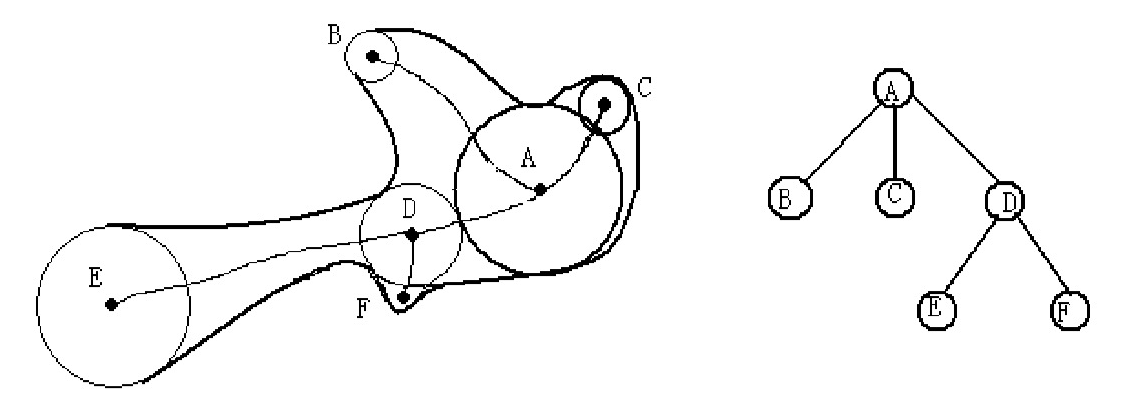
\includegraphics[width=0.5\linewidth]{tree}
            \caption{骨架树}
            \label{fig:tree}
        \end{figure}
        根据骨架树深度优先搜索产生的节点序列中的所有节点用其孩子数替换,替换后得到的新序列即为树描述符。例如,图\ref{fig:tree}的树描述符为(3,2,0,0,0,0)。

{\color{blue}骨架化代码}:\url{http://cs.smith.edu/~nhowe/research/code/}。

\subsubsection{SC}
    
    SC~\cite{belongie2002shape}(Shape context,形状上下文)是基于物体轮廓样本点进行描述的。
    
    {\color{blue}主要思想}:用直方图描述轮廓上点间的位置关系。
    
    {\color{blue}算法步骤}:
    \begin{enumerate}
        \item 边缘提取(如图\ref{fig:edge})。
           \begin{figure}
            \centering
              \begin{minipage}[t]{0.2\linewidth}
              \centering
              
\includegraphics[width=0.6\linewidth]{a1} 
              \caption{原始图像}
              \label{fig:org}
              \end{minipage}
              \begin{minipage}[t]{0.2\linewidth}
              \centering
              
\includegraphics[width=0.6\linewidth]{a-edge}
              \caption{边缘提取}
              \label{fig:edge}
              \end{minipage}
              \begin{minipage}[t]{0.2\linewidth}
              \centering
              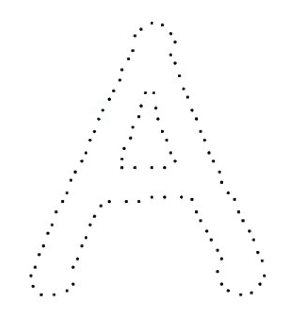
\includegraphics[width=0.6\linewidth]{a-point}
              \caption{采样点}
              \label{fig:point}
              \end{minipage}
            \end{figure}    
        \item 从边缘上均匀采样n个点,得到一个物体形状的点集合(如图\ref{fig:point})。
        \item 通过对数极坐标空间(如图\ref{fig:log})计算每个采样点与形状其他点之间的位置关系,采用直方图表示(如图\ref{fig:his})。n个采样点中,每个点都有一个直方图对其位置进行描述。
           \begin{figure}
            \centering
              \begin{minipage}[t]{0.4\linewidth}
              \centering
              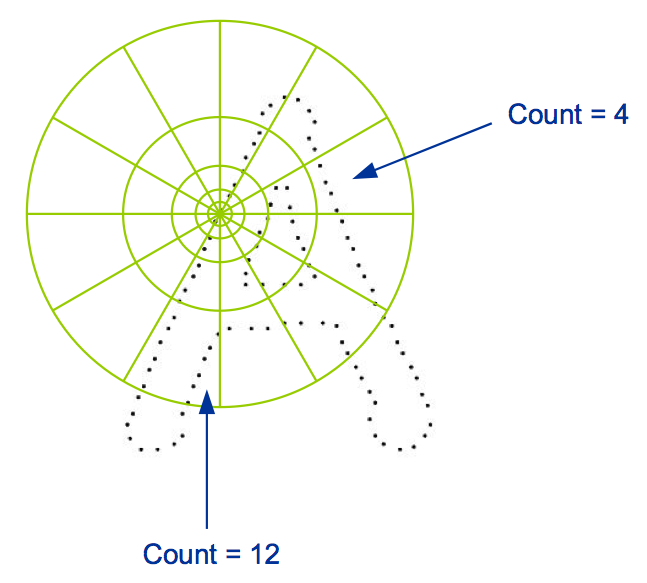
\includegraphics[width=0.6\linewidth]{a-log} 
              \caption{对数极坐标空间}
              \label{fig:log}
              \end{minipage}
              \begin{minipage}[t]{0.47\linewidth}
              \centering
              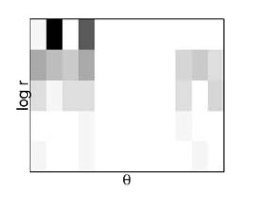
\includegraphics[width=0.6\linewidth]{his}
              \caption{直方图}
              \label{fig:his}
              \end{minipage}
            \end{figure}  
    \end{enumerate}
    但由于形状上下文不能很好地解决物体类内部之间的变形,因此采用基于内部距离的形状上下文~\cite{ling2007shape},内距离形状上下文中采用内距离代替欧式距离。
    
{\color{blue}内距离形状上下文代码}:\url{http://www.dabi.temple.edu/~hbling/code_data.htm}。


\subsubsection{哈尔特征(Haar-like features)}

Haar-like特征最早是由Oren等~\cite{oren1997pedestrian}应用于人脸表示,Viola和Jones~\cite{viola2001rapid}在此基础上,使用3种类型4种形式的特征。

Viola等提出的Harr-like特征如图~\ref{fig: Viola_Haar-like}:

\begin{figure}[!ht]
\centering
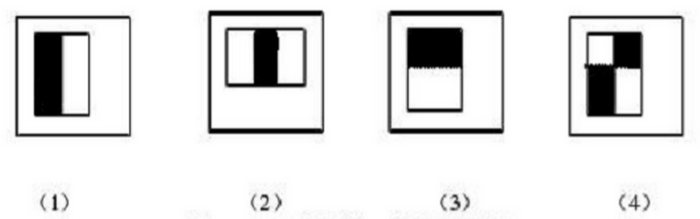
\includegraphics[width=4in]{Viola_Haar-like}
\caption{Viola提出的Haar-like特征}
\label{fig: Viola_Haar-like}
\end{figure}

将上面的任意一个矩形放到人脸区域上,然后,将白色区域的像素和减去黑色区域的像素和,得到的值我们暂且称之为人脸特征值,如果你把这个矩形放到一个非人脸区域,那么计算出的特征值应该和人脸特征值是不一样的,而且越不一样越好,所以这些方块的目的就是把人脸特征量化,以区分人脸和非人脸。

为了增加区分度,可以对多个矩形特征计算得到一个区分度更大的特征值,那么什么样的矩形特征怎么样的组合到一块可以更好的区分出人脸和非人脸呢,这就是AdaBoost算法要做的事了。

\subsection{其它特征}

\subsubsection{local symmetry}

Reisfeld等人~\cite{reisfeld1995context}发表的论文中有关于局部对称性的描述。

Isotropic Symmetry Operator:

\begin{figure}[!ht]
 \centering
 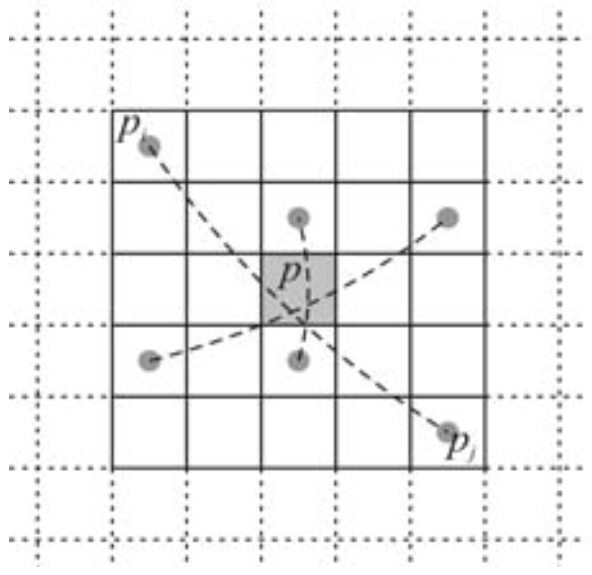
\includegraphics[width=3in]{ExamplesofPixelpairs}
\caption{用对称性算子来对像素对的梯度进行比较的三个例子}
\label{fig: ExamplesofPixelpairs}
\end{figure}

基于周围像素的灰度梯度,计算在给定点$p$处的对称性程度。如图~\ref{fig: ExamplesofPixelpairs}所示,点$p$处的对称性可以通过比较位于$p_i$和$p_j$处的像素对$i$和$j$的灰度梯度来度量,其中$p = (p_i  = p_j)/2$。每对像素对对点$p$处的局部对称性的贡献为
\begin{align}
c(i, j) = d(i, j, \sigma) \cdot p(i, j) \cdot m_i \cdot m_j
\end{align}
$m_i$是像素点$i$的梯度的模,$d(i, j, \sigma)$是当标准差为$\sigma$时,两个像素点间的距离的高斯加权函数,对称性
\begin{align}
p(i, j) = \Big(1-cos(\gamma_i+\gamma_j)\Big)\cdot \Big(1-cos(\gamma_i-\gamma_j)\Big)
\label{eq: SymmetryMeasurement}
\end{align}

其中,$\gamma_i = \theta_i-\alpha$,见图~\ref{fig: PixelpairContribution}。当点$p_i$、$p_j$关于点$p$对称时,$\gamma_i+\gamma_i=\pi$,式~(\ref{eq: SymmetryMeasurement})中的第一项取得最大值。如果只用第一项,会使得在直线边缘上的点取得较大的值,而这些点通常并不具有对称性。为了避免这个问题,又加入了第二项,表示具有相似梯度方向的像素对。最后,对所有像素对的贡献进行求和得到点$p$处的isotropic symmetry值
\begin{align}
M^{iso}(x, y) = \sum_{(i, j)\in \Gamma(p)} c(i, j)
\label{eq: IsotropicSymmetry}
\end{align}

\begin{figure}[!ht]
 \centering
 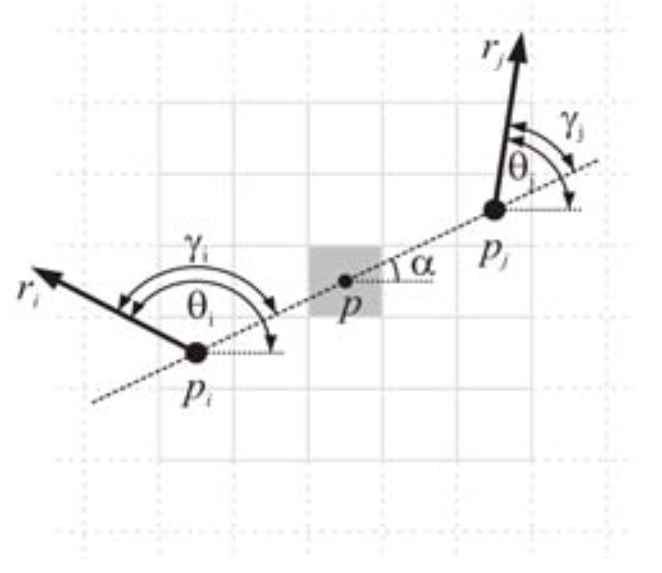
\includegraphics[width=3in]{PixelpairContribution}
\caption{每对像素对的贡献的几何表示}
\label{fig: PixelpairContribution}
\end{figure}

为了使symmetry operator对有多个对称轴的对称图案更敏感,Reisfeld等人~\cite{reisfeld1995context}又提出了radial symmetry operator,作为isotropic symmetry operator的扩展。首先,像素对的贡献的方向用$\varphi(i, j) = (\theta_i+\theta_j)/2$来计算。然后,对最大贡献为$c(i, j)$的像素对$(i, j)$,对称方向被确定为$\phi(p) = \varphi(i, j)$。这个值也用来提升有不相似方向的像素对的贡献
\begin{align}
M^{rad}= \sum_{(i, j)\in \Gamma(p)} c(i, j) \cdot sin^2(\varphi(i, j) - \phi(p))
\end{align}

\subsubsection{灰度特征}

1)灰度直方图
灰度直方图是灰度级函数,它表示图像中每种灰度级的像素的个数,反映图像中每种灰度出现的频率。灰度直方图的横坐标是灰度级,纵坐标是该灰度级出现的频率。

    \begin{lstlisting}[language=C++]
    imhist(I,n);
    \end{lstlisting}
    
2)灰度共生矩阵(GLCM)

灰度共生矩阵是对图像上保持某距离的两像素分别具有某种灰度的情况进行统计得到的。它不仅反映亮度的分布特性,也
反映具有同样亮度或接近亮度的像素之间的位置分布特性。对灰度共生矩阵的理解,需要明确几个概念:方向、偏移量和灰度共生矩阵的阶数。
\begin{description}
    \item[方向] 一般计算过程会分别选在几个不同的方向来进行,通常为0,45,90,135。
    \item[偏移量] 
    \item[灰度共生矩阵阶数] 灰度共生矩阵的阶数和灰度图像灰度值的阶数是一致的,即当灰度图像灰度值的阶数是$N$时,灰度共生矩阵为$N \times N$。
\end{description}

 取图像($N \times N$)中任意一点(x,y)及偏离它的另一点(x+a,y+b),设该点对的灰度值为(g1,g2)。令点(x,y)在整个画面上移动,则会得到各种(g1,g2)值,设灰度值的级数为256,则(g1,g2)的组合共有$256\times256$种(共生矩阵的大小)。对于整个画面,统计出每一种(g1,g2)值出现的次数,然后排列成一个方阵,在用(g1,g2)出现的总次数将它们归一化为出现的概率$P(g1,g2)$,这样的方阵称为灰度共生矩阵。
 
 为了能更直观的以共生矩阵描述纹理情况,从共生矩阵导出一下反映矩阵情况的参数,典型的有一下几种:
 \begin{description}
     \item[能量] 为灰度共生矩阵元素值的平方和,反映了图像灰度分布均匀程度和纹理粗细度。ASM值大表明一种较均一和规则变化的纹理模式。
         \begin{displaymath}
             ASM=\sum_{i=0}^{k}\sum_{j=0}^{k}G(i,j)^{2}
         \end{displaymath}
     \item[对比度] 反映了某个像素值及其领域像素值的亮度的对比情况。如果偏离对角线的元素有较大值,即图像亮度值变化很快,则CON会有较大取值。
         \begin{displaymath}
             CON=\sum_{i}\sum_{j}(i-j)^{2}G(i,j)
         \end{displaymath}
     \item[熵] 表示图像的信息量,当共生矩阵中所有元素有最大的随机性、空间共生矩阵中所有值几乎相等时,共生矩阵中元素分散分布时,熵较大。它表示了图像中纹理的非均匀程度或复杂程度。 
         \begin{displaymath}
             ENT=\sum_{i}\sum_{j}G(i,j)\log G(i,j)
         \end{displaymath}
     \item[自相关] 反应了图像纹理的一致性。如果图像中有水平方向纹理,则水平方向矩阵的COR大于其余矩阵的COR值。
         \begin{displaymath}
             COR=\frac{\sum_{i}\sum{j}[(ij)G(i,j)]-u_{i}u_{j}}{s_{i}s_{j}}
         \end{displaymath}
 \end{description}
 
    \begin{lstlisting}[language=C++]
    [glcm,SI] = graycomatrix(Img);
    \end{lstlisting}

\subsubsection{GIST}

GIST是一个全局描述子,主要用于场景分类。

\subsubsection{Harris-Laplace}

\subsubsection{GMM-HMM(Gaussian Mixture Model-Hidden Markov Model)}

{\color{blue}应用}:语音识别

\subsubsection{Gabor}

Gabor变换是D.Gabor 1946年提出的。Gabor变换属于加窗傅立叶变换,Gabor函数可以在频域不同尺度、不同方向上提取相关的特征。另外Gabor函数与人眼的生物作用相仿,所以经常用作纹理识别上,并取得了较好的效果。

Gabor滤波器是一个用于边缘检测的线性滤波器。用Gabor 函数形成的二维Gabor 滤波器具有在空间域和频率域同时取得最优局部化的特性,与人类生物视觉特性很相似,因此能够很好地描述对应于空间频率(尺度)、空间位置及方向选择性的局部结构信息。
同时,二维Gabor函数也类似于增强边缘以及峰、谷、脊轮廓等底层图像特征,这相当于增强了被认为是面部关键部件的眼睛、鼻子、嘴巴等信息,同时也增强了诸于黑痣、酒窝、伤疤等局部特征,从而使得在保留总体人脸信息的同时增强局部特性成为可能。它的小波特性说明了Gabor滤波结果是描述图像局部灰度分布的有力工具,因此,可以使用Gabor滤波来抽取图像的纹理信息。由于Gabor特征具有良好的空间局部性和方向选择性,而且对光照、姿态具有一定的鲁棒性,因此在人脸识别中获得了成功的应用。

{\color{blue}应用}:人脸识别、人脸表情识别、汉字识别

\subsubsection{DoG}


\subsubsection{Covariance Matrix}


\subsubsection{凸包}

\subsubsection{ICA(Independent Component Analysis)}

独立成分分析(Independent Component Analysis, ICA)是近年来出现的一种强有力的数据分析工具(Hyvarinen A, Karhunen J, Oja E, 2001; Roberts S J, Everson R, 2001)。1994年由Comon给出了ICA的一个较为严格的数学定义,其思想最早是由Heranlt和Jutten于1986年提出来的。ICA从出现到现在虽然时间不长,然而无论从理论上还是应用上,它正受到越来越多的关注,成为国内外研究的一个热点。特别是从应用角度看,它的应用领域与应用前景都是非常广阔的,目前主要应用于盲源分离、图像处理、语言识别、通信、生物医学信号处理、脑功能成像研究、故障诊断、特征提取、金融时间序列分析和数据挖掘等。
ICA是一种用来从多变量(多维)统计数据里找到隐含的因素或成分的方法,被认为是主成分分析(Principal Component Analysis, PCA)和因子分析(Factor Analysis)的一种扩展。对于盲源分离问题,ICA是指在只知道混合信号,而不知道源信号、噪声以及混合机制的情况下,分离或近似地分离出源信号的一种分析过程。





田奇

binary feature descriptors

\subsubsection{Binary SIFT (BSIFT) – Zhou, TIP 2014}

\subsubsection{COGE - PCM 2013 Best Paper, Mao , 2013}

\subsubsection{Ultra-Short Binary Descriptor (USB) – Zhang S., TIP , 2014}

\subsubsection{Topology-Preserving Hashing – Zhang L., MM 2012}


\section{学习算法}

\subsection{贝叶斯学习}

贝叶斯学习是由英国学者T. Bayesian(贝叶斯)~\cite{mr1763essay}于1763年提出的一种归纳推理的理论。

贝叶斯学习的基本公式如下:
\begin{align}
P(A|B) = \frac{P(B|A)P(A)}{P(B)}
\end{align}

\subsection{SVM方法}

SVM(Support Vector Machine,支持向量机)是一种有监督的统计学习方法,能够最小化经验误差和最大化几何边缘,被称为最大间隔分类器,可用于分类与回归分析。最早的相关论文为美国贝尔实验室(Bell Lab., USA)的Corinna Cortes和Vladimir Vapnik等人于1995年在Machine Learning杂志上提出~\cite{cortes1995support},被引用次数已经超过17600次。

{\color{blue}代码}:SVMlight\footnote{\url{http://svmlight.joachims.org/}}和LibSVM\footnote{\url{http://www.csie.ntu.edu.tw/~cjlin/libsvm}}

SVM是一种典型的两类分类器,即它只回答属于正类还是负类的问题。当遇到多类别的时候,一般采取如下两种策略:
\begin{itemize}
    \item 一对多法:训练时依次把某个类别的样本归为一类,其他剩余的样本归为另一类,这样$k$个类别的样本就构造出了$k$个SVM。分类时将未知样本分类为具有最大分类函数值的那类。
    
    比如我们有5个类别,第一次就把类别1的样本定为正样本,其余2,3,4,5的样本合起来定为负样本,这样得到一个两类分类器,它能够指出一篇文章是还是不是第1类的;第二次我们把类别2 的样本定为正样本,把1,3,4,5的样本合起来定为负样本,得到一个分类器,如此下去,我们可以得到5个这样的两类分类器(总是和类别的数目一致)。到了有文章需要分类的时候,我们就拿着这篇文章挨个分类器的问:是属于你的么?是属于你的么?哪个分类器点头说是了,文章的类别就确定了。这种方法的好处是每个优化问题的规模比较小,而且分类的时候速度很快(只需要调用5个分类器就知道了结果)。但有时也会出现两种很尴尬的情况,例如拿一篇文章问了一圈,每一个分类器都说它是属于它那一类的,或者每一个分类器都说它不是它那一类的,前者叫分类重叠现象,后者叫不可分类现象。分类重叠倒还好办,随便选一个结果都不至于太离谱,或者看看这篇文章到各个超平面的距离,哪个远就判给哪个。不可分类现象就着实难办了,只能把它分给第6个类别了。更要命的是,本来各个类别的样本数目是差不多的,但“其余”的那一类样本数总是要数倍于正类(因为它是除正类以外其他类别的样本之和嘛),这就人为的造成了上一节所说的“数据集偏斜”问题。
    \item 一对一法:其做法是在任意两类样本之间设计一个SVM,因此$k$个类别的样本就需要设计$\frac{k(k-1)}{2}$个SVM。当对一个未知样本进行分类时,最后得票最多的类别即为该未知样本的类别。LibSVM中的多类分类就是根据这个方法实现的。
    
    每次选一个类的样本作正类样本,而负类样本则变成只选一个类,这就避免了偏斜。因此过程就是算出这样一些分类器,第一个只回答“是第1类还是第2类”,第二个只回答“是第1类还是第3类”,第三个只回答“是第1类还是第4类”,如此下去,你也可以马上得出,这样的分类器应该有$\frac{5\times 4}{2}=10$个(通式是,如果有k个类别,则总的两类分类器数目为$\frac{k(k-1)}{2}$)。虽然分类器的数目多了,但是在训练阶段(也就是算出这些分类器的分类平面时)所用的总时间却比“一类对其余”方法少很多,在真正用来分类的时候,把一篇文章扔给所有分类器,第一个分类器会投票说它是“1”或者“2”,第二个会说它是“1”或者“3”,让每一个都投上自己的一票,最后统计票数,如果类别“1”得票最多,就判这篇文章属于第1类。这种方法显然也会有分类重叠的现象,但不会有不可分类现象,因为总不可能所有类别的票数都是0。看起来够好么?其实不然,想想分类一篇文章,我们调用了多少个分类器?10个,这还是类别数为5的时候,类别数如果是1000,要调用的分类器数目会上升至约500,000个(类别数的平方量级)。
    \item 层次支持向量机:还是像一对一方法那样来训练。在分类时可以先问分类器“1对5”(意思是它能够回答“是第1类还是第5类”),如果它回答5,我们就再问“2对5”这个分类器,如果它还说是“5”,我们就继续问下去,就可以得到分类结果。好处在哪?我们其实只调用了4个分类器(如果类别数是k,则只调用k-1个),分类速度飞快,且没有分类重叠和不可分类现象!缺点在哪?假如最一开始的分类器回答错误(明明是类别1的文章,它说成了5),那么后面的分类器是无论如何也无法纠正它的错误的(因为后面的分类器压根没有出现“1”这个类别标签),其实对下面每一层的分类器都存在这种错误向下累积的现象。
    \end{itemize}

\subsection{K-means}

\subsection{Decision tree}

\subsection{EM(Expectation Maximization Algorithm)}
期望最大算法(Expectation Maximization Algorithm,EM)是一种从不完全数据或有数据丢失的数据集中求解概率模型参数的最大似然估计方法。

{\color{blue}算法步骤}:
\begin{enumerate}
    \item 初始化分布参数。
    \item 重复以下步骤直到收敛:
        \begin{enumerate}
            \item E步骤:估计未知参数的期望值,给出当前的参数估计。
            \item M步骤:重新估计分布参数,以使得数据的似然性最大,给出未知变量的期望估计。
        \end{enumerate}
\end{enumerate}

\subsection{KNN}

K最近邻分类算法,是一个理论上比较成熟的方法,也是最简单的机器学习算法之一。该方法的思路是:如果一个样本在特征空间中的k个最相 似(即特征空间中最邻近)的样本中的大多数属于某一个类别,则该样本也属于这个类别。由于KNN方法主要靠周围有限的邻近的样本,而不是靠判别类域的方 法来确定所属类别的,因此对于类域的交叉或重叠较多的待分样本集来说,KNN方法较其他方法更为适合。

\subsection{ELM(极限学习机)}

ELM算法~\cite{huang2004extreme}是新加坡南洋理工大学的黄广斌教授提出来的。

{\color{blue}代码}:\url{http://www.ntu.edu.sg/home/egbhuang/}

\subsection{集成学习(Ensemble learning)}

集成学习(Ensemble learning)是使用一系列学习器进行学习,并使用某种规则把各个学习结果进行整合从而获得比单个学习器更好的学习效果的一种机器学习方法。

{\color{blue}主要思路}:

在对新的实例进行分类的时候,把若干个单个分类器集成起来,通过对多个分类器的分类结果进行某种组合来决定最终的分类,以取得比单个分类器更好的性能。

\subsubsection{AdaBoost}

AdaBoost,是英文``Adaptive Boosting''(自适应增强)的缩写,由Yoav Freund和Robert Schapire在1995年提出。它的自适应在于:前一个基本分类器分错的样本会得到加强,加权后的全体样本再次被用来训练下一个基本分类器。同时,在每一轮中加入一个新的弱分类器,直到达到某个预定的足够小的错误率或达到预先指定的最大迭代次数。

{\color{blue}主要步骤}:
\begin{enumerate}
    \item 初始化训练数据的权值分布。如果有N个样本,则每一个训练样本最开始时都被赋予相同的权值:$\frac{1}{N}$。
    \item 训练弱分类器。具体训练过程中,如果某个样本点已经被准确地分类,那么在构造下一个训练集中,它的权值就被降低;相反,如果某个样本点没有被准确地分类,那么它的权值就得到提高。然后,权值更新过的样本集被用于训练下一个分类器,整个训练过程如此迭代地进行下去。
    \item 将各个训练得到的弱分类器组合成强分类器。各个弱分类器的训练过程结束后,加大分类误差率小的弱分类器的权重,使其在最终的分类函数中起着较大的决定作用,而降低分类误差率大的弱分类器的权重,使其在最终的分类函数中起着较小的决定作用。
\end{enumerate}

相关资料:\url{http://cs.nju.edu.cn/zhouzh/zhouzh.files/publication/top10chapter.pdf}

\subsubsection{Bagging}

{\color{blue}主要思路}:

让学习算法训练多轮,每轮的训练集由从初始的训练集中随机取出的n个训练样本组成,某个初始训练样本在某轮训练集中可以出现多次或根本不出现,训练之后可得到一个预测函数序列$h\_1, \dots, h\_n$,最终的预测函数H对分类问题采用投票方式。

随机森林(Random Forest)是一种采用决策树作为基预测器的集成学习方法,2001年由Breiman~\cite{breiman2001random}提出,结合Bagging和随机子空间理论,集成众多决策树进行预测,通过各个决策树的预测值进行平均或投票,得到最终预测结果。

“视觉机器学习20讲”中提供了随机森林的源代码,是c与matlab的混合编程,但是只有在windows下编译好了的文件,在mac下无法跑。

DRFI方法中用到随机森林\footnote{\url{https://code.google.com/p/randomforest-matlab/}}学习方法,下载下来解压后是在randomforest-matlab文件夹中,其中又包含两个文件夹,一个是RF\_Class\_C,用来做分类的,另一个是RF\_Reg\_C,用来做回归的。

RF\_Class\_C文件夹中需要对.cpp文件进行编译,生成mexmaci64文件,这一步可以通过在终端输入make mex命令实现。但是可能由于我电脑中的fortran版本不行,编译总是出错,目前还没有解决,后来在网页上\footnote{\url{https://code.google.com/p/randomforest-matlab/issues/detail?id=54}}搜到了已编译好的mexmaci64文件,可以直接拿过来用。

tutorial\_ClassRF.m文件列举了10个例子,展示了用不同的参数跑随机森林学习算法的不同结果。

\subsubsection{Gasen}

GASEN~\cite{zhou2002ensembling}(基于遗传算法的选择性集成学习算法)。随机生成若干权向量,权向量的每个分量对应了一个个体学习器,这些权向量被遗传算法进化,得到一个最优权向量,它表示了各个体学习器在构成集成时的“重要性”,据此进行个体的选择。该方法是建立在遗传算法基础上,由于遗传算法计算效率低,使得 GASEN 计算量更大。

{\color{blue}代码}:\url{http://lamda.nju.edu.cn/Default.aspx?Page=code_GASEN&NS=&AspxAutoDetectCookieSupport=1}

\section{技术路线和方案}

\subsection{技术路线}

在设计浮游动物分类系统过程中,需要完成特征和分类器的选择,我们的技术路线如图~\ref{fig:TechnicalRoute}。

特征选取:根据浮游动物的形态特征和计算机视觉中分类识别常用的经典特征,我们选取的特征如图~\ref{fig:TechnicalRoute}。

分类器的训练:根据经典学习方法和集成学习,我们选择的学习算法如图~\ref{fig:TechnicalRoute}。

    \begin{figure}[!ht]
    \centering
    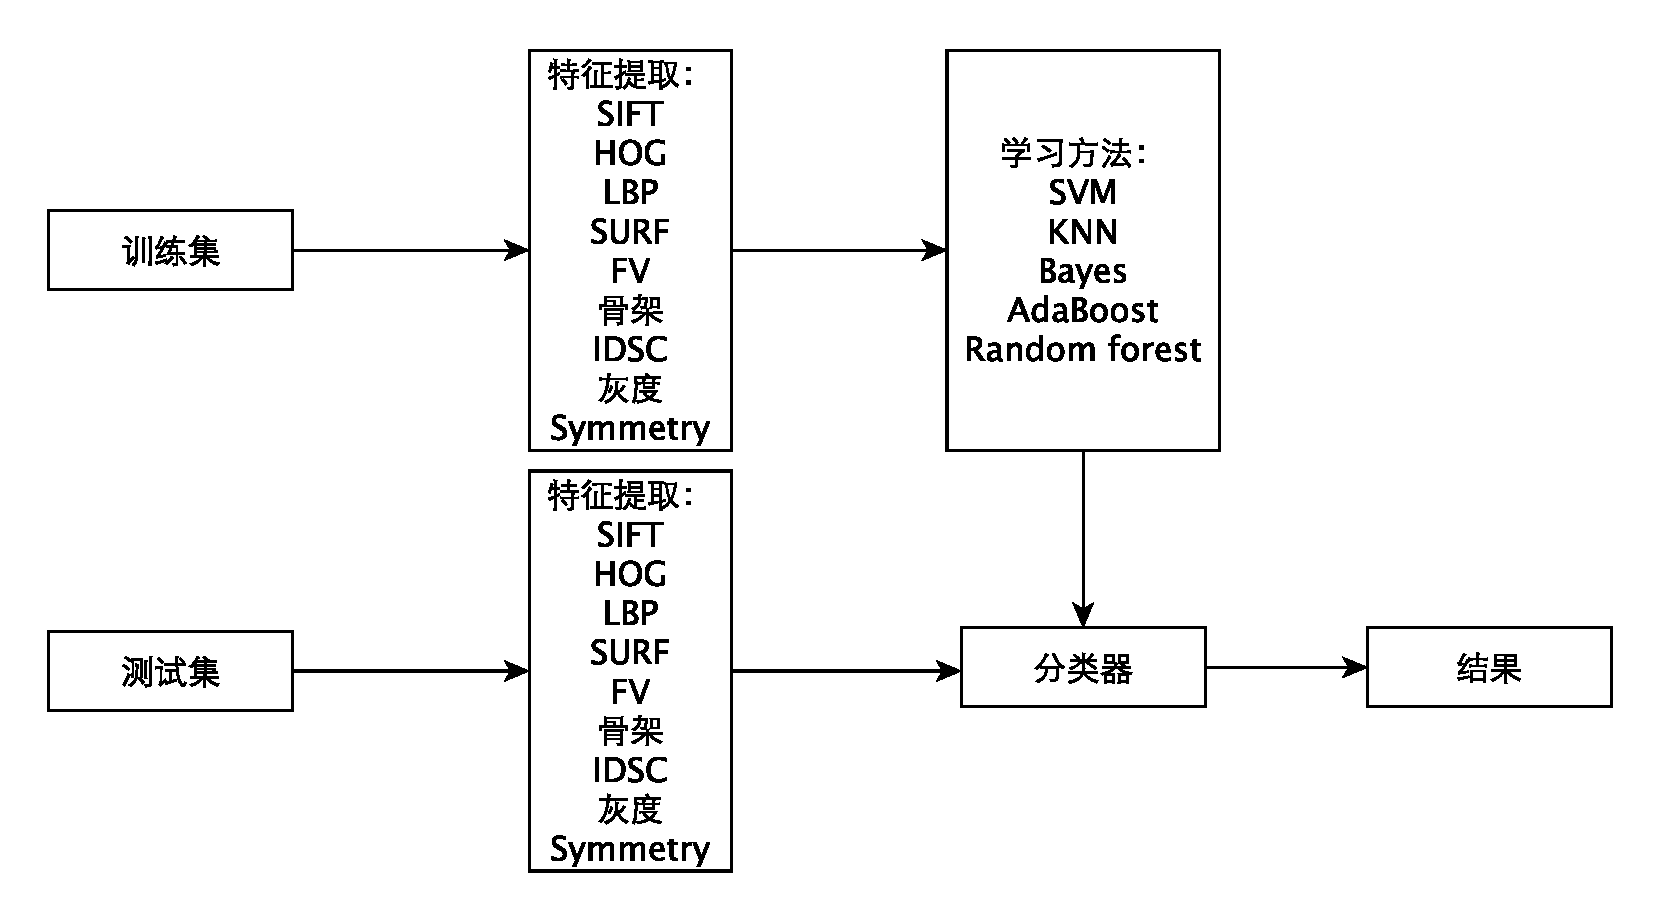
\includegraphics[width=4in]{TechnicalRoute}
    \caption{技术路线}
    \label{fig:TechnicalRoute}
    \end{figure}

\section{实验}

\subsection{HOG+SVM}
在实验中,针对SVM核函数选用了Linear核和RBF核。
\begin{itemize} 
\item Linear核:主要用于线性可分的情形。参数少,速度快,对于一般数据,分类效果已经很理想了。
\item RBF核:主要用于线性不可分的情形。参数多,分类结果非常依赖于参数。
\end{itemize}
实验中,将图像resize为$64 \times 64$,以整幅图像作为一个窗口提取HOG特征,其中块(block)选用$16 \times 16$,单元(cell)选用$8 \times 8$。

\subsubsection{HOG+C-SVC Linear}
实验得到的\textbf{re-substitution Confusion Matrix}(自身验证自身)如图~\ref{fig: Train-CM-HOG-SVM-Linear}:
\begin{figure}[!ht]
\centering
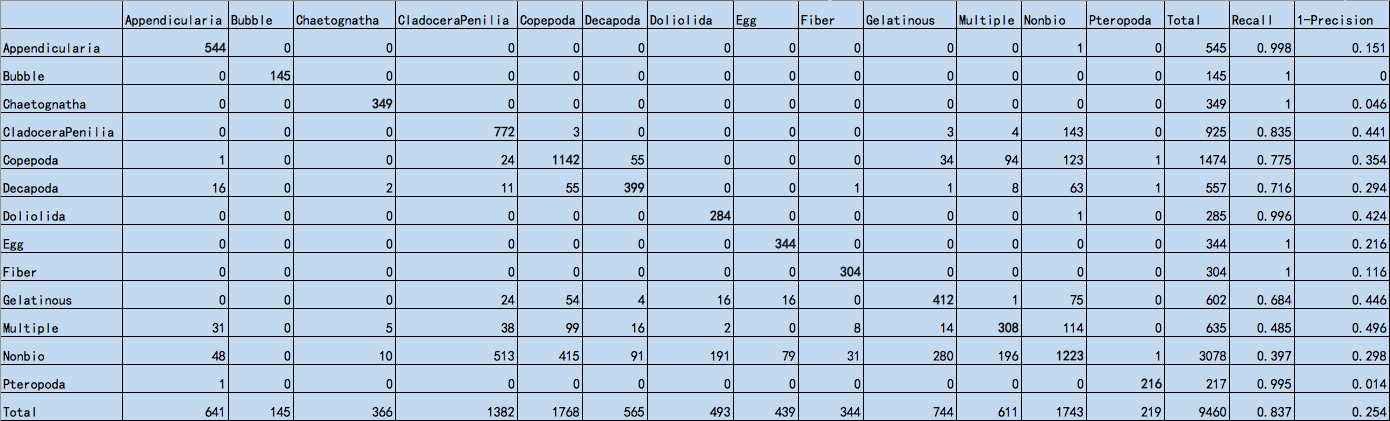
\includegraphics[width=1.0\linewidth]{Train-CM-HOG-SVM-Linear}
\caption{混淆矩阵(训练集与测试集相同)}
\label{fig: Train-CM-HOG-SVM-Linear}
\end{figure}

对测试集进行预测得到的混淆矩阵如图~\ref{fig: Test-CM-HOG-SVM-linear}:
\begin{figure}[!ht]
\centering
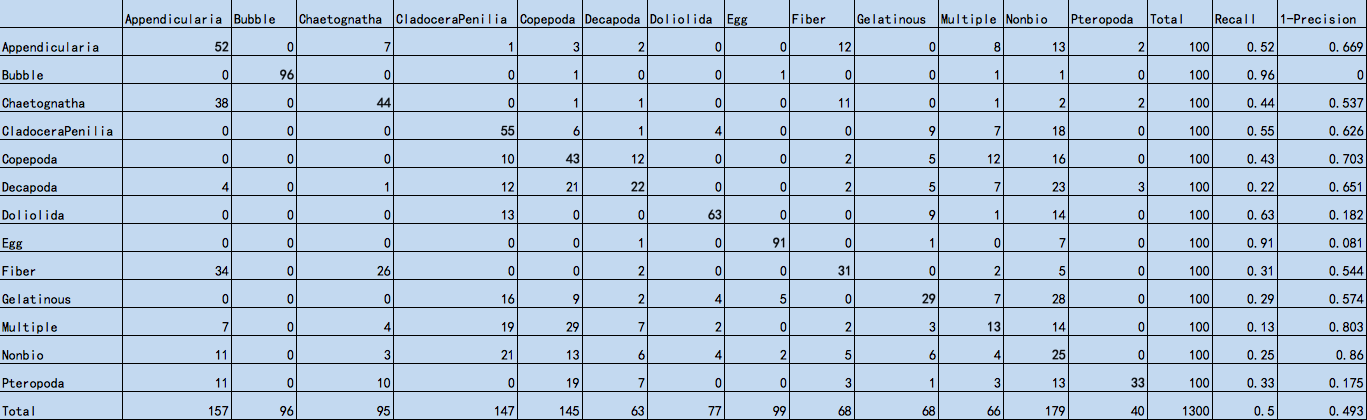
\includegraphics[width=1.0\linewidth]{Test-CM-HOG-SVM-linear}
\caption{混淆矩阵(训练集与测试集不同)}
\label{fig: Test-CM-HOG-SVM-linear}
\end{figure}

\subsubsection{C-SVC RBF}
实验得到的\textbf{re-substitution Confusion Matrix}(自身验证自身)如图~\ref{fig: Train-CM-HOG-SVM-RBF}:
\begin{figure}[!ht]
\centering
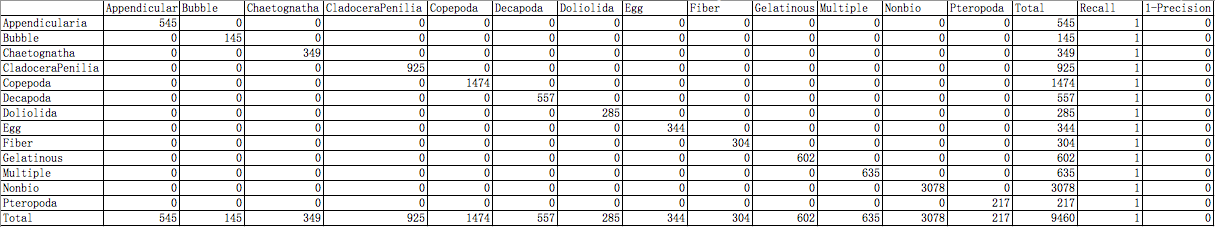
\includegraphics[width=1.0\linewidth]{Train-CM-HOG-SVM-RBF}
\caption{混淆矩阵(训练集与测试集相同)}
\label{fig: Train-CM-HOG-SVM-RBF}
\end{figure}

对测试集进行预测得到的混淆矩阵如图~\ref{fig: Test-CM-HOG-SVM-RBF}:
\begin{figure}[!ht]
\centering
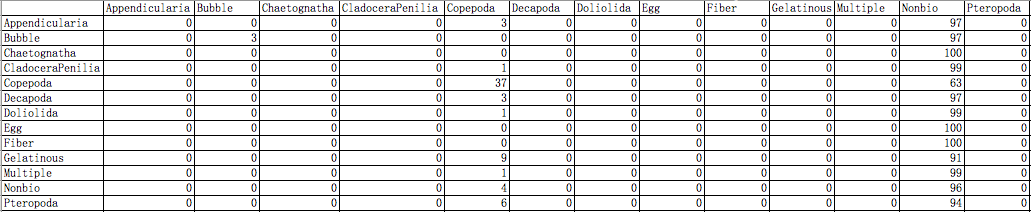
\includegraphics[width=1.0\linewidth]{Test-CM-HOG-SVM-RBF}
\caption{混淆矩阵(训练集与测试集不同)}
\label{fig: Test-CM-HOG-SVM-RBF}
\end{figure}

\subsection{LBP+SVM}
SVM核函数也选用了Linear核和RBF核。
实验中,将图像划分为$16 \times 16$的区域,统计每一个区域内的LBP直方图(直方图的bin设置为256)。

\subsubsection{C-SVC Linear}
实验得到的\textbf{re-substitution Confusion Matrix}(自身验证自身)如图~\ref{fig: Train-CM-LBP-SVM-linear}:
\begin{figure}[!ht]
\centering
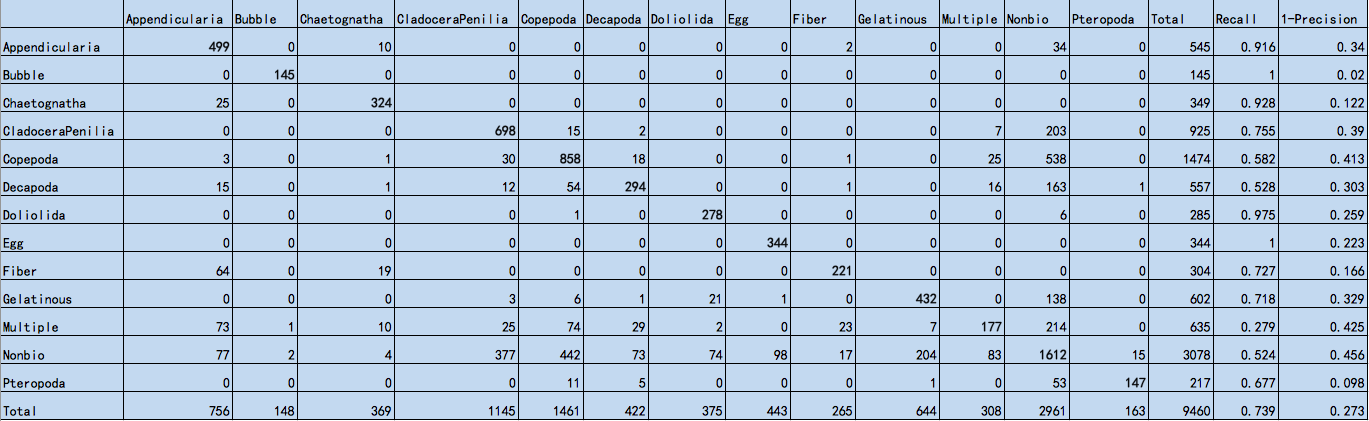
\includegraphics[width=1.0\linewidth]{Train-CM-LBP-SVM-linear}
\caption{混淆矩阵(训练集与测试集相同)}
\label{fig: Train-CM-LBP-SVM-linear}
\end{figure}

对测试集进行预测得到的混淆矩阵如图~\ref{fig: Test-CM-LBP-SVM-linear}:
\begin{figure}[!ht]
\centering
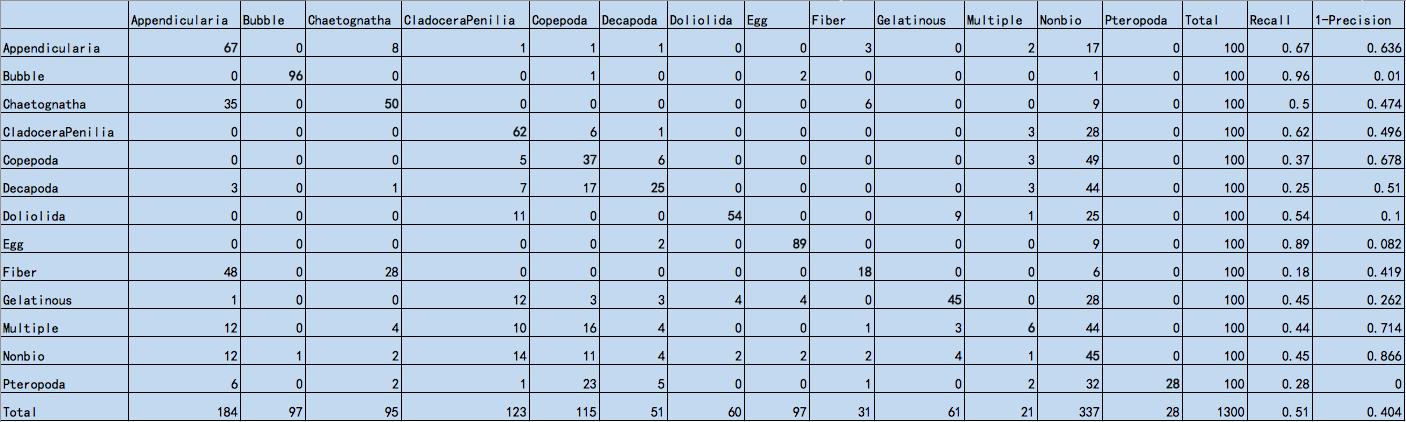
\includegraphics[width=1.0\linewidth]{Test-CM-LBP-SVM-linear}
\caption{混淆矩阵(训练集与测试集不同)}
\label{fig: Test-CM-LBP-SVM-linear}
\end{figure}

\subsubsection{C-SVC RBF}
实验得到的\textbf{re-substitution Confusion Matrix}(自身验证自身)如图~\ref{fig: Train-CM-LBP-SVM-RBF}:
\begin{figure}[!ht]
\centering
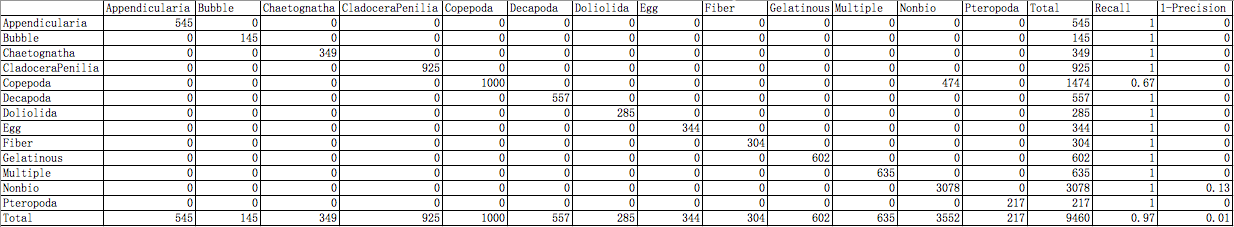
\includegraphics[width=1.0\linewidth]{Train-CM-LBP-SVM-RBF}
\caption{混淆矩阵(训练集与测试集相同)}
\label{fig: Train-CM-LBP-SVM-RBF}
\end{figure}

\subsection{SIFT+BoW+SVM}

\subsection{实验总结}

\subsubsection{遇到的问题}
\begin{enumerate}
    \item SIFT实验结果不对,几乎全都分类错误。
    \item 交叉验证代码没有找到,找到的交叉验证代码都不是MATLAB和C的,没有跑通。
    \item 没有来得及调参数,对参数的影响效果也不是很了解。
    \item 用测试集跑出来的实验结果在Multiple和Nonbio类上效果最差,Bubble和Egg上效果最好。
\end{enumerate}

\subsubsection{方案}

20150706$\sim$20150710 用三个经典特征(HOG, SIFT, LBP)和SVM分类器分别完成对浮游动物的分类,并对分类结果进行评价分析。

20150713$\sim$20150717 根据我们上周遇到的问题,决定在这周对这些问题进行进一步研究:
\begin{enumerate}
    \item 用MATLAB版的SIFT和bag of word进行实验。
    \item 调整特征以及SVM分类器的参数,分析对效果的影响;用交叉验证对SVM进行优化,分析效果。
    \item 打算索要完整的20类浮游动物的数据集。
    \item 调试交叉验证的程序。
\end{enumerate}

20150720$\sim$20150724 仍然用三个经典特征(HOG、SIFT、LBP),分类器换为随机森林和ELM进行实验。

在回家之前,初步实现一套浮游动物分类系统。

\bibliographystyle{plain}

\bibliography{ResearchPlan} %参考文献

\end{document}
